\documentclass[mathserif,t]{beamer}
%\usepackage{Sweave}                                                       
%http://tex.stackexchange.com/questions/105613/footer-in-beamer. Check this out. Frankfurt template.
%http://tex.stackexchange.com/questions/39345/piecewise-highlighting-in-beamer-presentation
%https://joerglenhard.wordpress.com/2011/08/01/beamer-customization-colors/
\usepackage{amssymb,bm,mathtools,amsmath}                                                      
\usepackage{graphicx,caption,float}
\usepackage[UKenglish]{isodate} % for: \today                             
\cleanlookdateon                % for: \today

\usepackage{natbib}
\bibliographystyle{plain}

\def\wl{\par\vspace{\baselineskip}\noindent}                             
\def\beginmyfig{\begin{figure}[ht]\begin{center}}                          
\def\endmyfig{\end{center}\end{figure}}                                   

\def\prodl#1#2#3{\prod\limits_{#1=#2}^{#3}}                               
\def\suml#1#2#3{\sum\limits_{#1=#2}^{#3}}                                 
\def\ds{\displaystyle}                                                    
\def\tbf#1{\textbf{#1}}
\def\inv{^{\raisebox{.2ex}{$\scriptscriptstyle-1$}}}
\def\pm{^{\raisebox{.2ex}{$\scriptscriptstyle\prime$}}}
\newcommand{\norm}[1]{\left\lVert#1\right\rVert}
\newcommand{\p}[1]{\left(#1\right)}
\newcommand{\bk}[1]{\left[#1\right]}
\newcommand{\bc}[1]{ \left\{#1\right\} }
\newcommand{\abs}[1]{ \left|#1\right| }
\def\I{\bm I}
\def\N{\mathcal N}
\newcommand{\mat}{ \begin{pmatrix} }
\newcommand{\tam}{ \end{pmatrix} }


% My Beamer Stuff
  \geometry{vmargin=0.3in} % Formating the top bar
  \newcommand{\m}[1]{\mathbf{\bm{#1}}} % Serif bold math

  % My Color Stuff
  \usepackage{xcolor} % http://en.wikibooks.org/wiki/LaTeX/Colors
                      % http://latexcolor.com/
    \definecolor{grey}{rgb}{0.15, 0.15, 0.15} % Sets default color. CHANGE THIS!
    \definecolor{pumpkin}{rgb}{1.0, 0.46, 0.09}
    \definecolor{darktan}{rgb}{1.0, 0.66, 0.07}
    \definecolor{coral}{rgb}{1.0, 0.5, 0.31}
    \definecolor{burlywood}{rgb}{0.98, 0.82 0.6}
    \pagecolor{grey}% Sets the bar color.

  \def\mylitecolor{pumpkin}         % Bullet Color.       CHANGE THIS!
  \def\mycolor{\color{pumpkin}}     % Frame Title Color.  CHANGE THIS!
  \def\mydarkcolor{\color{pumpkin}} % Figure Color.       CHANGE THIS!
    \def\frametitle#1{\vspace{-.32in{\mycolor\textbf{\Large#1}}}}
    \setbeamercolor{itemize item}{fg=\mylitecolor}
    \setbeamercolor{enumerate item}{fg=\mylitecolor}
    \setbeamercolor{itemize subitem}{fg=\mylitecolor}
    \setbeamercolor{itemize subsubitem}{fg=\mylitecolor}
    \setbeamercolor{title}{fg=\mylitecolor}
    \setbeamercolor{footlinecolor}{bg=black!93,fg=\mylitecolor}
    \setbeamercolor{author}{fg=burlywood}
    \setbeamercolor{date}{fg=burlywood}
    \setbeamercolor{institute}{fg=burlywood}

    \usepackage[T1]{fontenc}
    \DeclareCaptionFont{figcol}{\mydarkcolor} %color of the word Figure: in figure captions
    \captionsetup{
      font=scriptsize,
      labelfont={bf,figcol,scriptsize}%,textfont={black}
    }
  \def\hline{ \textcolor{grey}{\hrulefill}\\ }

  % Beamer Footer Stuff:
  %http://tex.stackexchange.com/questions/26476/add-footer-text-to-all-slides-in-beamer
  %http://tex.stackexchange.com/questions/105613/footer-in-beamer
  \beamertemplatenavigationsymbolsempty
  \setbeamertemplate{footline}{
    \hbox{
      \hspace{-.17cm}
      \begin{beamercolorbox}[ht=2mm,dp=8.2mm,leftskip=.3cm,rightskip=.3cm]{footlinecolor}%
        \insertauthor\hfill\insertshorttitle\hfill\insertframenumber/\inserttotalframenumber
      \end{beamercolorbox}
    }
  }

%%%%% Example for embedding images: %%%%%%%%%%%%%%%%%%%%%%%%%%%%%%%%%%%%%%%%%%%%%%%%%%%%%%%%%%%%
%%%\frame{
%%%  \frametitle{How to embed images:}
%%%  \beginmyfig
%%%    \includegraphics[scale=.21]{path/to/file.pdf}
%%%    \caption{Put Caption Here}
%%%  \endmyfig
%%%  \footnote{\tiny \url{https://www.luiarthur.github.com} }
%%%}
% End of Header. Start below beamer below. %%%%%%%%%%%%%%%%%%%%%%%%%%%%%%%%%%%%%%%%%%%%%%%%%%%%%

% defs for this assignment:

\begin{document}
% My Title: {
\def\mytitle{\textbf{Introduction to the Indian Buffet Process}}
  \title[IBP]{\mytitle}
  \author[Arthur Lui]{Arthur Lui}
  \institute{
    AMS\\
    UC Santa Cruz
  }
  {
    \setbeamercolor{background canvas}{bg=grey}
    \frame{\titlepage}
  }
%}

\frame{ %
  \frametitle{Motivation}
  \vspace{15mm}

  Factor Analysis
  \vspace{5mm}
  \begin{itemize}
      \item $\bm{ X = F\Lambda + \epsilon}$, where only $\bm X$ is observed
  \end{itemize}
  \vspace{10mm}

  Latent binary feature allocation models
  \vspace{5mm}
  \begin{itemize}
      \item $\bm{ X = ZA + \epsilon}$, where only $\bm X$ is observed
      \item $\bm Z$ is a binary matrix
      \item IBP($\alpha$) Prior on $\bm Z$ 
  \end{itemize}
}

\frame{ %
  \frametitle{Traditional Formulation}
  \vspace{5mm}

  Griffiths et al. \cite{griffiths2011indian} introduced the
  IBP as follows:
  \vspace{5mm}

  Let $\bm Z$ be a $N\times K$ matrix such that
  $$
  \begin{array}{rclcl}
    z_{ik} &\mid& \pi_k  &\sim& \text{Bernoulli}(\pi_k) \\
    \pi_k  &\mid& \alpha &\sim& \text{Beta}\p{\frac{\alpha}{K},1} \\ 
  \end{array}
  $$
  for $i=1,\cdots N$ and $k=1,\cdots, K$, and where $\alpha$ is positive. \\

  Then as $K\rightarrow \infty$, $\bm Z \sim \text{IBP}(\alpha)$.
  It can be shown that
  $$
  \text{P}(\bm Z) = \frac{\alpha^{K_+}}{\prodl{h}{1}{2^N-1} 
                          {K_h}!} 
                          \exp\{-\alpha H_N\}\prodl{k}{1}{K_+}
                                       \frac{(N-m_k)!(m_k-1)!}{N!},
  $$

  where $H_N$ is the harmonic number, 
  $\suml{i}{1}{N}i^{-1}$, $K_+$ is
  the number of non-zero columns in $\bm Z$, $m_k$ is the $k^{th}$
  column sum of $\bm Z$, and $K_h$ the number of columns having
  history $h$ (some binary number).
}


\frame{ %
  \frametitle{Why is it called the Indian Buffet Process?}
  \vspace{5mm}
  \beginmyfig
    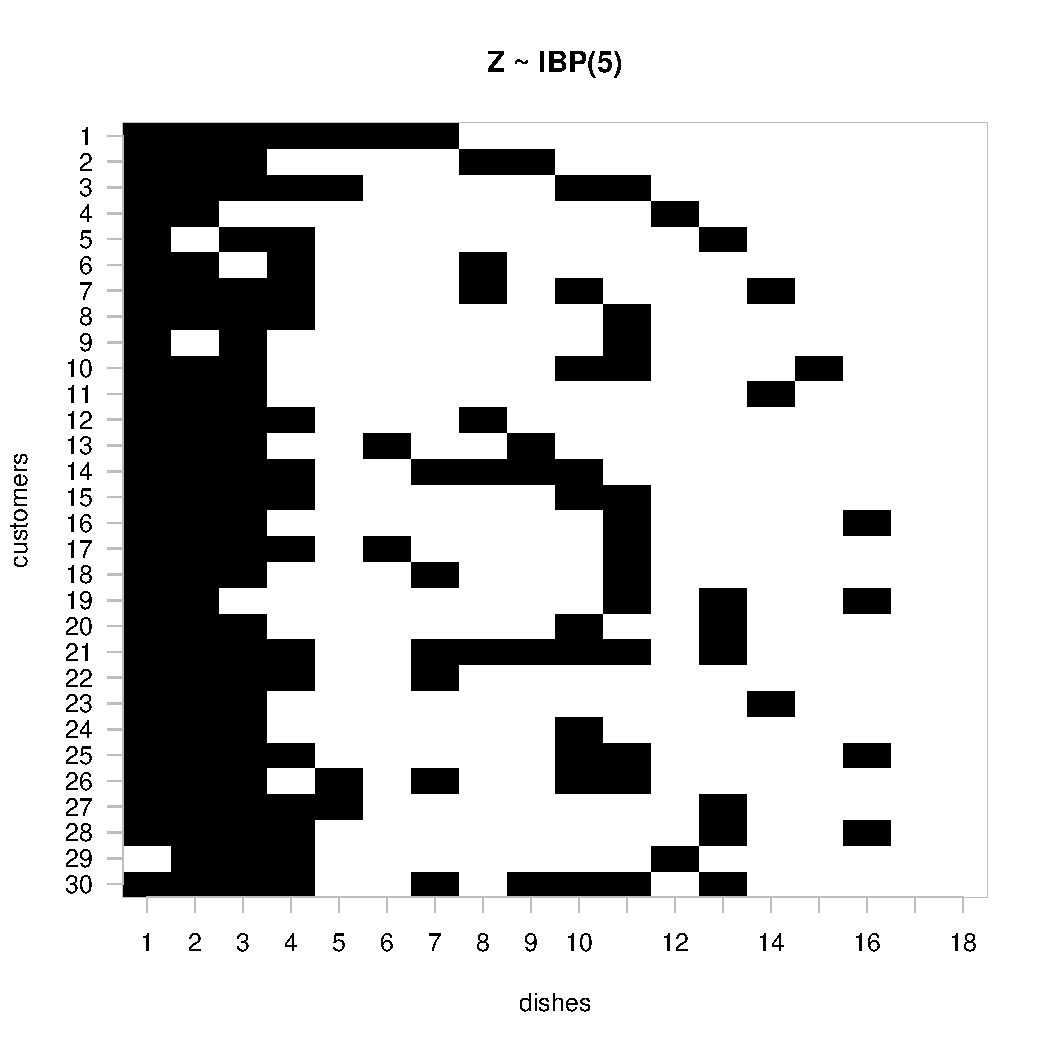
\includegraphics[scale=.4]{../img/Z.pdf}
    %\caption{}
  \endmyfig
}

\frame{ %
  \frametitle{Why is it called the Indian Buffet Process?}
  \vspace{10mm}

  In the IBP, a customer ($i$) taking a dish ($k$) is analogous to an
  observation possessing a feature. This is indicated by setting the value of
  $z_{ik}$ to 1 if the customer takes the dish, and 0 otherwise. \\

  \vspace{5mm}
  An IBP($\alpha$) for $N$ observations can be simulate as follows:
  \begin{enumerate}
    \item The $1^{st}$ customer takes Poisson($\alpha$) number of dishes
    \item For customers $i=2 \text{ to } N$,
    \begin{itemize}
      \item For each previously sampled dish,
            customer $i$ takes dish $k$ with probability $m_k / i$
      \item after sampling the last sampled dish, customer $i$ samples 
            Poisson($\alpha/i$) new dishes
    \end{itemize}
  \end{enumerate}

  \vspace{5mm}
  It can be shown that a matrix generated by this process 
  has the same pmf up to a proportionality constant as the
  previous pmf.
}

% Draws from IBP
\frame{ %
  \frametitle{What does a sample look like?}
  \vspace{5mm}
  \beginmyfig
    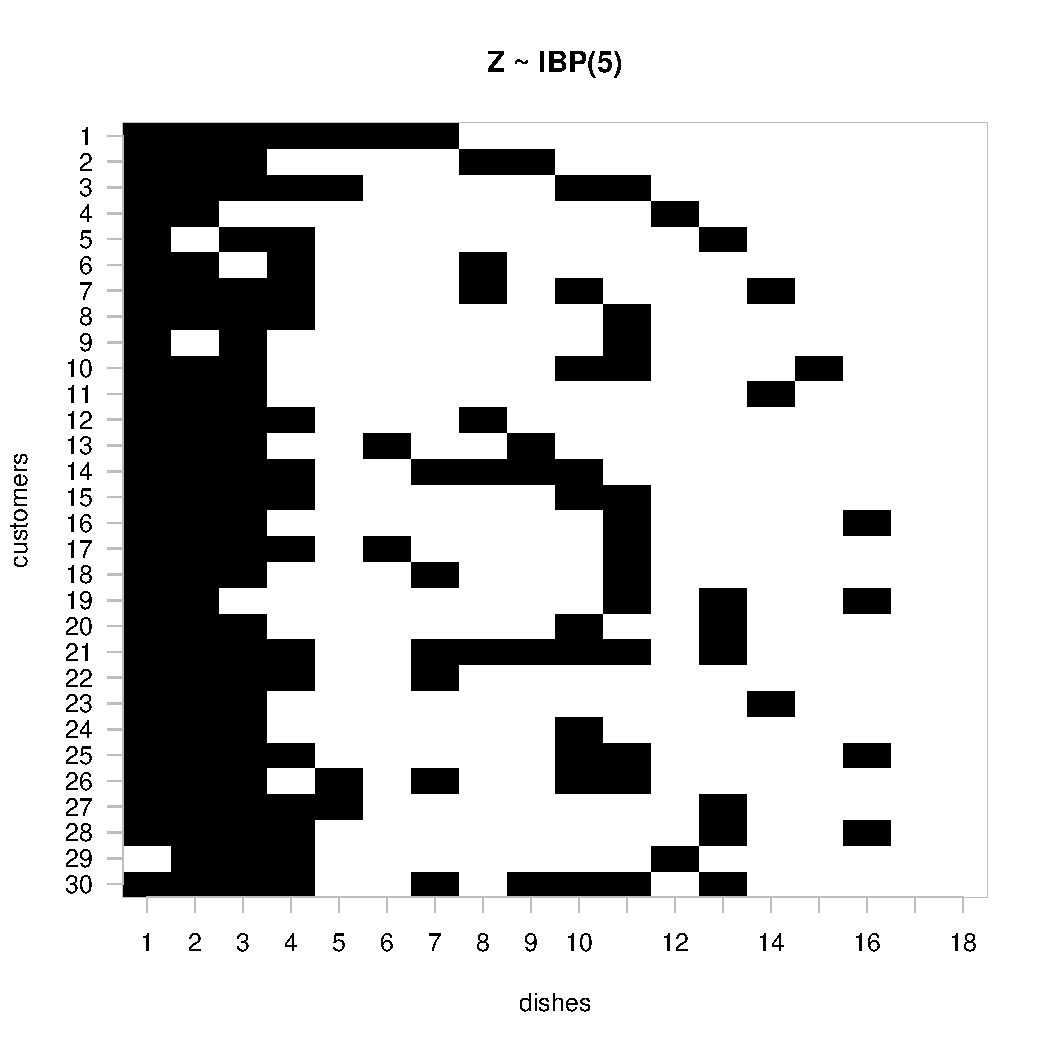
\includegraphics[scale=.4]{../img/Z.pdf}
    %\caption{Put Caption Here}
  \endmyfig
}
\frame{ %
  \frametitle{What does a sample look like?}
  \vspace{5mm}
  \beginmyfig
    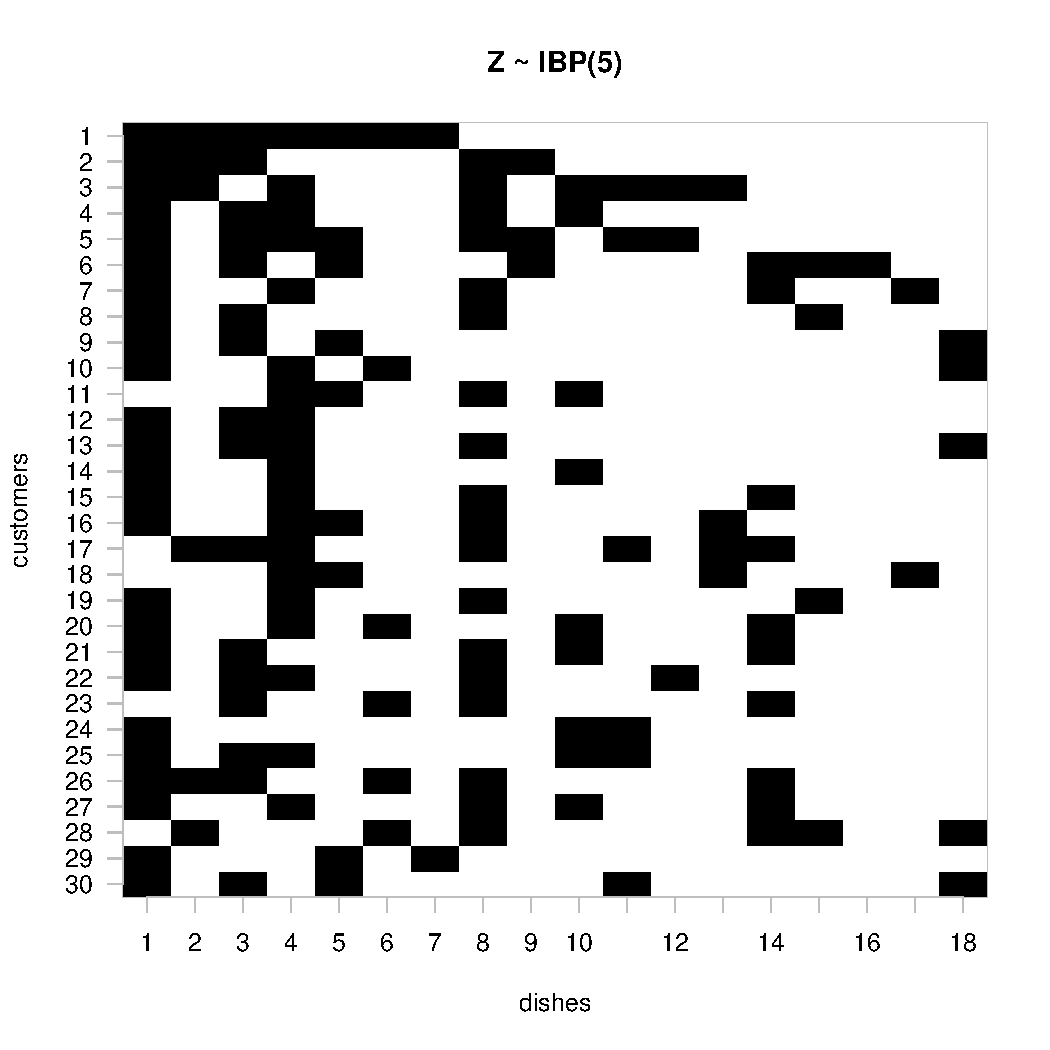
\includegraphics[scale=.4]{../img/Z2.pdf}
    %\caption{Put Caption Here}
  \endmyfig
}
\frame{ %
  \frametitle{What does a sample look like?}
  \vspace{5mm}
  \beginmyfig
    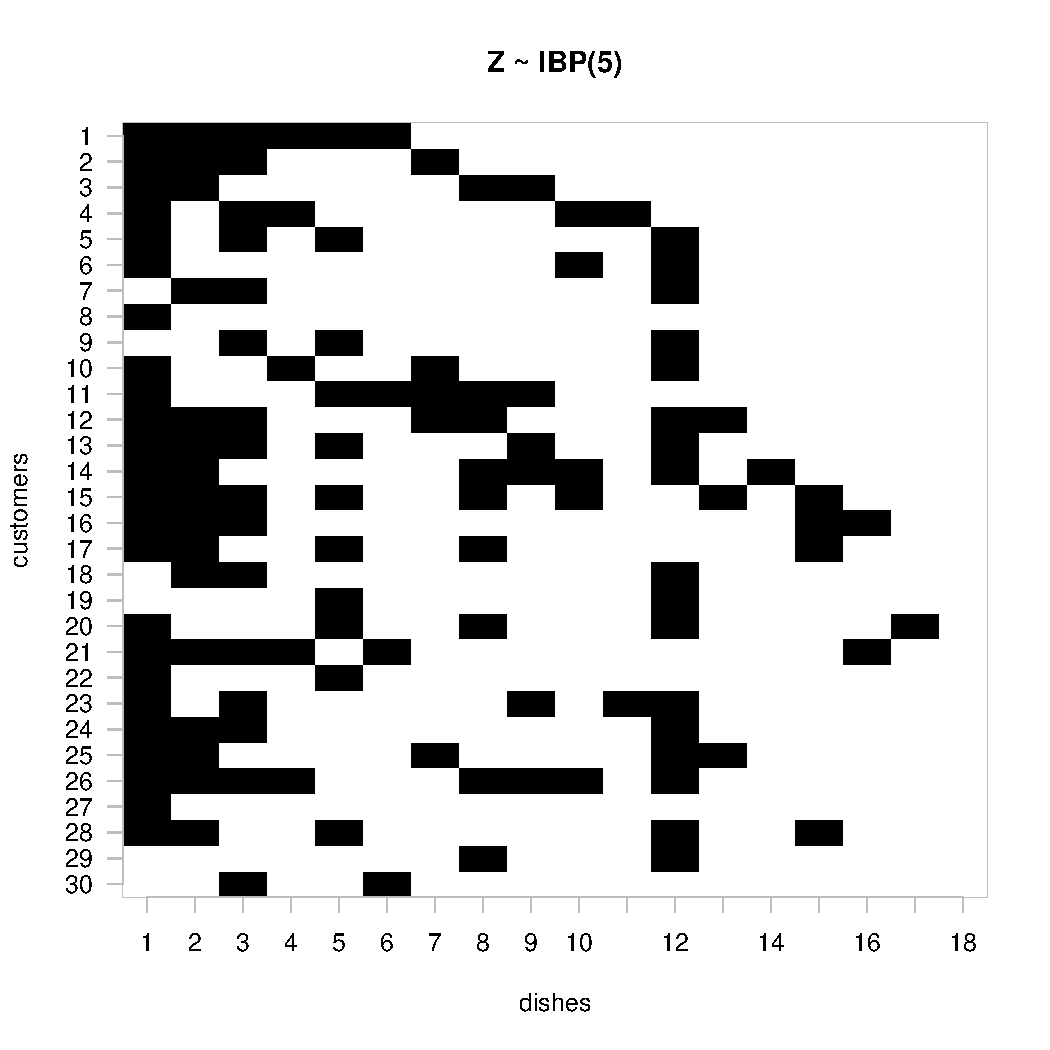
\includegraphics[scale=.4]{../img/Z3.pdf}
    %\caption{Put Caption Here}
  \endmyfig
}

% IBP Expectation
\frame{ %
  \frametitle{What does a sample look like?}
  \vspace{5mm}
  \beginmyfig
    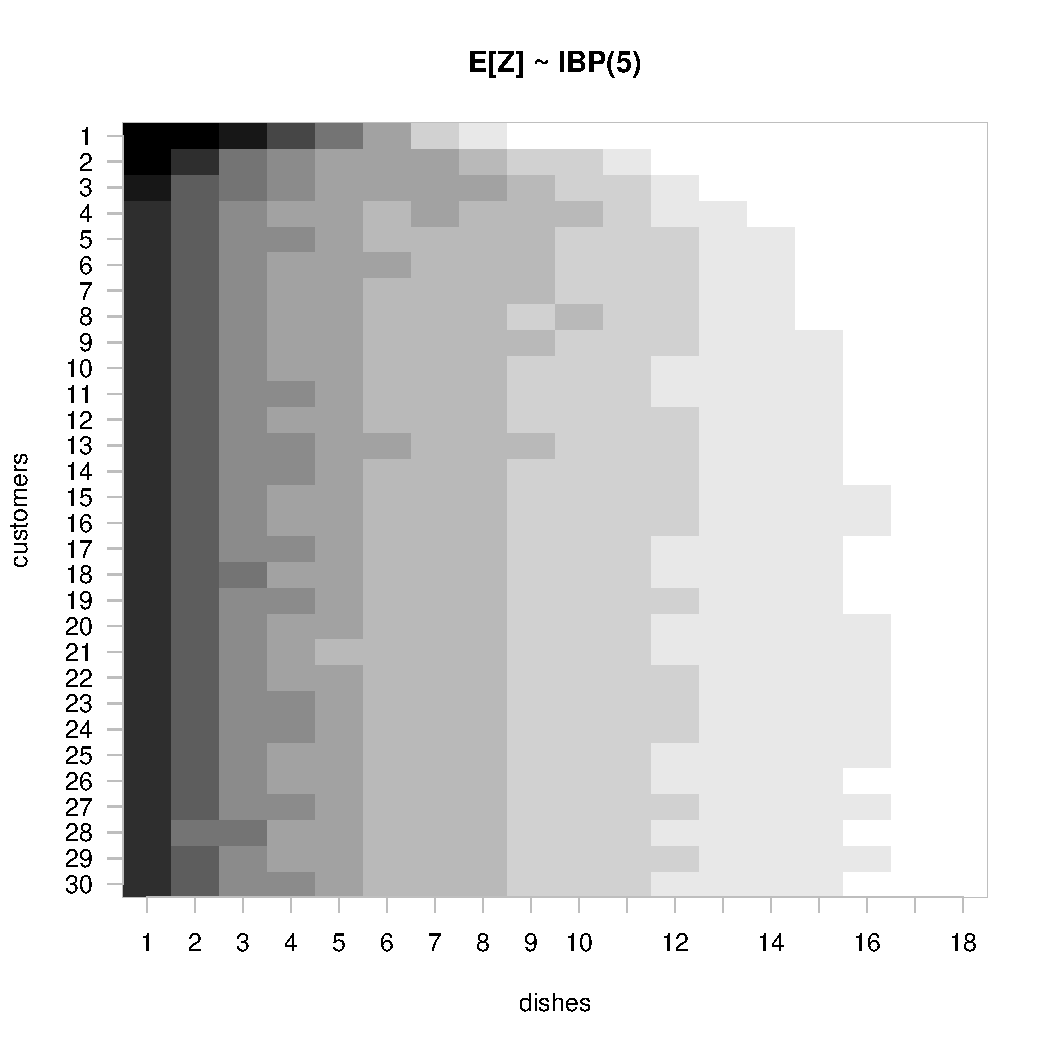
\includegraphics[scale=.4]{../img/EZ.pdf}
    %\caption{Put Caption Here}
  \endmyfig
}

\frame{ %
  \frametitle{Stick-breaking Construction}
  \vspace{5mm}

  Teh et al. \cite{teh2007stick} introduced the stick-breaking
  construction for the IBP:

  $$
  \begin{aligned}
    v_l &\sim \text{Beta}(\alpha,1) \\
    z_{ik} &\sim \text{Bernoulli}(\prod_{l=1}^k v_l) \\
  \end{aligned}
  $$

  \vspace{5mm}
  This representation was adopted in the dependent IBP 
  by Williamson et al. \cite{williamson2010dependent}, 
  which assumes dependence between ``customers''.
}


\frame{ %
  \frametitle{Toy Example}
  \vspace{5mm}

  \beginmyfig
    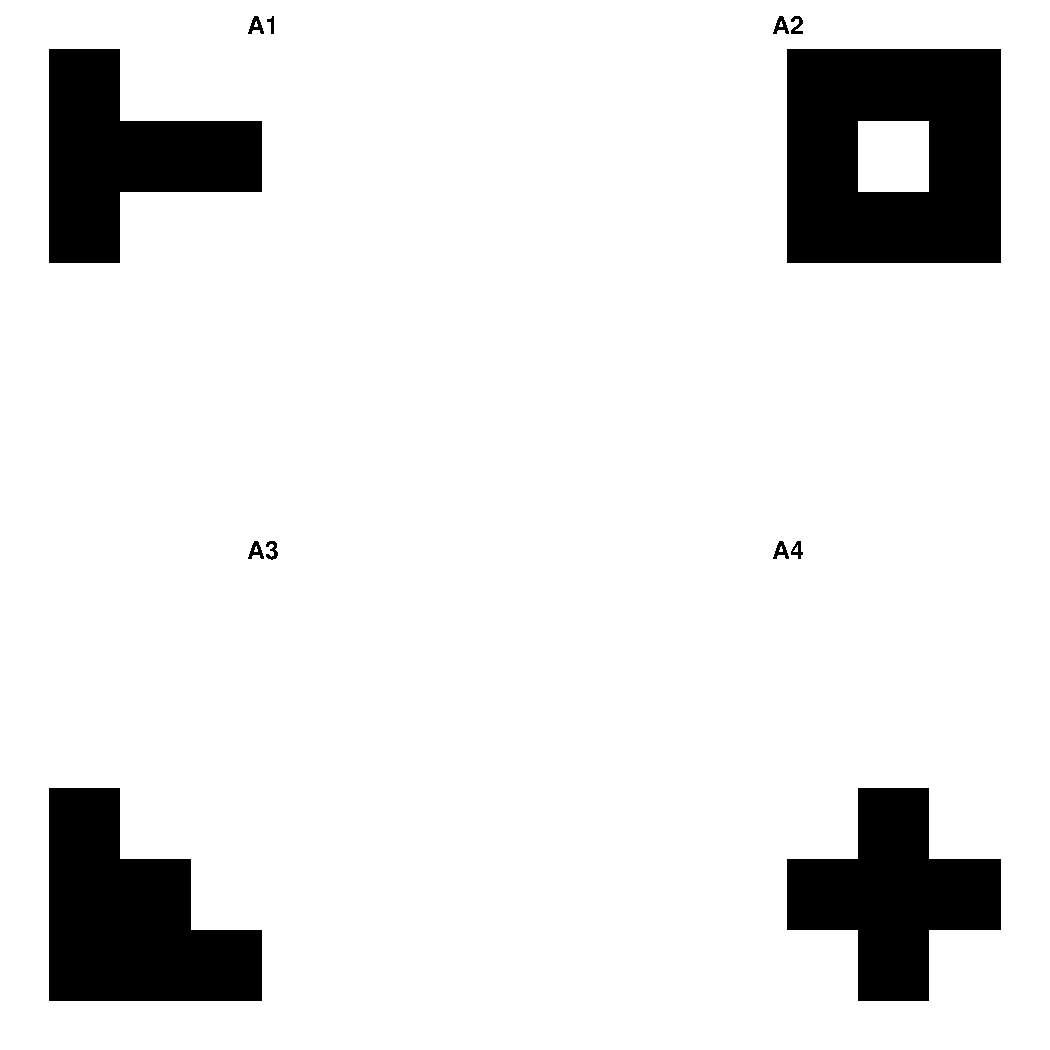
\includegraphics[scale=.4]{../img/A.pdf}
    \caption{Latent features in a latent feature model}
  \endmyfig
}

\frame{ %
  \frametitle{Toy Example}
  \vspace{5mm}

  Generate observation matrix $\bm X$ from a random binary
  matrix $\bm Z$, the latent features matrix $\bm A$, and 
  gaussian noise $\bm \epsilon$. i.e. generate

  $$
  \bm {X = ZA + \epsilon}
  $$

  where $X$ is $N\times D$, $Z$ is $N\times K$, and 
  $A$ is $K \times D$. $(N=100, D=36, K=4)$

  \vspace{5mm}
  Each row in $\bm A$ is a 36-dimesnional vector which
  represents one of the $6\times6$ image.

  \vspace{5mm}
  $Z_{ik}=1$ indicates that feature $k$ is in observation $i$.
  Each observation can be comprised of multiple features.

  \vspace{5mm}
  \textbf{Goal:} Recover $\bm Z$ and $\bm A$.
}

\frame{ %
  \frametitle{Toy Example}
  \vspace{5mm}

  \textbf{Model}
  \vspace{5mm}

  $$
  \begin{aligned}
    \bm X \mid \bm Z, \bm A &\sim \N(\bm{ZA}, \sigma^2_X I_N, \sigma^2_XI_D) \\
    \bm A &\sim \N(\bm 0, \sigma^2_A\I_K,\sigma^2_A\I_D) \\
    \bm Z \mid \alpha &\sim \text{IBP}(\alpha) \\
    \alpha &\sim \text{Gamma}(a,b)\\
  \end{aligned}
  $$

  Priors can be placed on $\sigma_A^2$ and $\sigma_X^2$.
  \vspace{5mm}

  Note that $\bm A$ can be analytically integrated out, to 
  yield $p(\bm{X\mid Z})$. A posterior mean for $\bm A$ 
  is then 

  $$
  E[\bm A \mid \bm X] = \p{\bm Z' \bm Z + 
  \frac{\sigma_X^2}{\sigma_A^2}\I}^{-1} \bm {Z'X}.
  $$
}

\frame{ %
  \frametitle{Toy Example}
  \vspace{5mm}

  \textbf{Model}
  \vspace{5mm}

  $$
  \begin{aligned}
    \bm X \mid \bm Z, \bm A &\sim \N(\bm{ZA}, \sigma^2_X I_N, \sigma^2_XI_D) \\
    \bm A &\sim \N(\bm 0, \sigma^2_A\I_K,\sigma^2_A\I_D) \\
    z_{ik} &\sim \text{Bernoulli}\p{\prod_{l=1}^k v_l} \\
    v_l &\sim \text{Beta}(\alpha,1) \\
    \alpha &\sim \text{Gamma}(a,b)\\
  \end{aligned}
  $$

  Priors can be placed on $\sigma_A^2$ and $\sigma_X^2$.
  \vspace{5mm}

}


\frame{ %
  \frametitle{Results}
  \vspace{5mm}
  \beginmyfig
    
\includegraphics[scale=.4]{../img/post.pdf}
    %\caption{Put Caption Here}
  \endmyfig
}


\frame{ %
  \frametitle{Estimating $K$}
  \vspace{5mm}

  \begin{enumerate}
    \item Reversible jump?
    \item slice sampling
    \item Fixing $K$ at a sufficiently large value
  \end{enumerate}
}


\frame{ %
  \frametitle{Applications}
  \vspace{15mm}

  \begin{enumerate}
    \item genomics
      \begin{itemize}
        \item $\bm Z$ is $J$ by $K$
        \item $j \in \bc{1,\cdots,J}$ represents a genetic marker
        \item $k \in \bc{1,\cdots,K} $ represents a latent feature
        \item The vector $\bm{z}_k$ is then a combination of genes (phenotype)
      \end{itemize}
    \item modeling protein interactions
    \item modeling relational data
    \item[] $\vdots$
  \end{enumerate}
}

\begin{frame}[allowframebreaks]
  \frametitle{References}
  \bibliography{ibp}
\end{frame}

\end{document}
% To compile:
%  $ pdflatex *.tex; pdflatex *.tex
